\documentclass{article}

\usepackage{fancyhdr}
\usepackage{extramarks}
\usepackage{amsmath,mathrsfs,amssymb}
\usepackage{amsthm}
\usepackage{amsfonts}
\usepackage{tikz}
\usepackage[plain]{algorithm}
\usepackage{algpseudocode}
\usepackage{graphicx}
\usepackage{pgfplots}
\usepackage{xfrac}
\usepackage{caption}
\usepackage{epstopdf}
\usepackage{siunitx}
\usepackage{circuitikz} % Required for the drawing of circuit diagrams
\usepackage{float}

\usetikzlibrary{automata,positioning}

%
% Basic Document Settings
%

\topmargin=-0.45in
\evensidemargin=0in
\oddsidemargin=0in
\textwidth=6.5in
\textheight=9.0in
\headsep=0.25in

\linespread{1.1}

\pagestyle{fancy}
\lhead{\hmwkAuthorName}
\chead{\hmwkClass\ : \hmwkTitle}
\rhead{\firstxmark}
\lfoot{\lastxmark}
\cfoot{\thepage}

\renewcommand\headrulewidth{0.4pt}
\renewcommand\footrulewidth{0.4pt}

\setlength\parindent{0pt}

%
% Create Problem Sections
%

\newcommand{\enterProblemHeader}[1]{
    \nobreak\extramarks{}{Problem \arabic{#1} continued on next page\ldots}\nobreak{}
    \nobreak\extramarks{Problem \arabic{#1} (continued)}{Problem \arabic{#1} continued on next page\ldots}\nobreak{}
}

\newcommand{\exitProblemHeader}[1]{
    \nobreak\extramarks{Problem \arabic{#1} (continued)}{Problem \arabic{#1} continued on next page\ldots}\nobreak{}
    \stepcounter{#1}
    \nobreak\extramarks{Problem \arabic{#1}}{}\nobreak{}
}

\setcounter{secnumdepth}{0}
\newcounter{partCounter}
\newcounter{homeworkProblemCounter}
\setcounter{homeworkProblemCounter}{1}
\nobreak\extramarks{Problem \arabic{homeworkProblemCounter}}{}\nobreak{}

%
% Homework Problem Environment
%
% This environment takes an optional argument. When given, it will adjust the
% problem counter. This is useful for when the problems given for your
% assignment aren't sequential. See the last 3 problems of this template for an
% example.
%
\newenvironment{homeworkProblem}[1][-1]{
    \ifnum#1>0
        \setcounter{homeworkProblemCounter}{#1}
    \fi
    \section{Problem \arabic{homeworkProblemCounter}}
    \setcounter{partCounter}{1}
    \enterProblemHeader{homeworkProblemCounter}
}{
    \exitProblemHeader{homeworkProblemCounter}
}

%
% Homework Details
%   - Title
%   - Due date
%   - Class
%   - Section/Time
%   - Instructor
%   - Author
%

\newcommand{\hmwkTitle}{Assignment\ 1}
\newcommand{\hmwkDueDate}{August 07, 2016}
\newcommand{\hmwkClass}{Electrical Machines \& Power Systems}
\newcommand{\hmwkClassTime}{}
\newcommand{\hmwkClassInstructor}{Dr. Kamal Debnath}
\newcommand{\hmwkAuthorName}{S.Reynolds (262538)}

%
% Title Page
%

\title{
    \vspace{2in}
    \textmd{\textbf{\hmwkClass:\ \hmwkTitle}}\\
    \normalsize\vspace{0.1in}\small{Due\ on\ \hmwkDueDate\ at 3:10pm}\\
    \vspace{0.1in}\large{\textit{\hmwkClassInstructor\ \hmwkClassTime}}
    \vspace{3in}
}

\author{\textbf{\hmwkAuthorName}}
\date{}

\renewcommand{\part}[1]{\textbf{\large Part \Alph{partCounter}}\stepcounter{partCounter}\\}

%
% Various Helper Commands
%

% Useful for algorithms
\newcommand{\alg}[1]{\textsc{\bfseries \footnotesize #1}}

% For derivatives
\newcommand{\deriv}[1]{\frac{\mathrm{d}}{\mathrm{d}x} (#1)}

% For partial derivatives
\newcommand{\pderiv}[2]{\frac{\partial}{\partial #1} (#2)}

% Integral dx
\newcommand{\dx}{\mathrm{d}x}

% Alias for the Solution section header
\newcommand{\solution}{\textbf{\large Solution}}

% Probability commands: Expectation, Variance, Covariance, Bias
\newcommand{\E}{\mathrm{E}}
\newcommand{\Var}{\mathrm{Var}}
\newcommand{\Cov}{\mathrm{Cov}}
\newcommand{\Bias}{\mathrm{Bias}}

\DeclareMathOperator{\sinc}{sinc}

\begin{document}

\maketitle

\pagebreak

%%%%%%%%%%%%%%%%%%%%%%%%%%%%%%%%%%%%%%%%%%%%%%%%%%%%%%%%%%%%%%%%%%%%%%%%%%%%%%%%%%%%%%%%%%%%%%%%%%%%%%%%%%%%%%%%%%%%%%
% Question 1
%%%%%%%%%%%%%%%%%%%%%%%%%%%%%%%%%%%%%%%%%%%%%%%%%%%%%%%%%%%%%%%%%%%%%%%%%%%%%%%%%%%%%%%%%%%%%%%%%%%%%%%%%%%%%%%%%%%%%% 

\begin{homeworkProblem}
    
    An electrical load consists of three resistances connected in series-parallel. The series resistor, $R_1$, has a value of 1.6 $\si{\ohm}$, and the two parallel connectd resistors are reated at 4 $\si{\ohm}$ and 6 $\si{\ohm}$ respectively. A 12 $\si{\volt}$ battery supplies the load. A picture of the circuit is shown below.
	\begin{figure}[h]
		\centering
	 	\ctikzset{bipoles/length=0.8cm}
	 	\begin{circuitikz}
	 		\draw
	 		(0,0) to [battery,l=$12\ V$, i=$i$] (0,2)node[above]{A}
	 		to[R,l=$R_1$, *-*] (2,2)node[above]{B} 
	 		to[R, l=$R_2$] (2,0) -- (0,0)
	 		(2,2) -- (4,2)
	 		to[R, l=$R_3$] (4,0) -- (2,0)
	 		;
	 	\end{circuitikz}
	\end{figure}
    
    \textbf{1.1.1}\\
    
    The equivalent resistance of the circuit is given by:
    \begin{align*}
	    R_{eq} 	&= R_1 + R_2||R_3\\
			    &= 1.6 + (\frac{1}{4} + \frac{1}{6})^{-1}\\
			    &= 4 \si{\ohm}
    \end{align*}
    
    Now, by Ohm's law, we get that:
    \begin{center}
	    \fbox{$i = \frac{V}{R_{eq}} = \frac{12}{4} = 3 \si{\ampere}$}\\
    \end{center}
    
    Now, taking care to ensure that we use the passive sign convention for power, we get that the power from the source is given by:
    \begin{center}
	    \fbox{$P = -i \cdot v = -3 \cdot 12 = -36 \si{\watt}$}
    \end{center}
    
    \vspace{1cm}
    
    \textbf{1.1.2}\\
    
    The current through the resistor $R_1$ is:\\
    \begin{center}
    	\fbox{$i_{R_1} = 3 \si{\ampere}$}
    \end{center}
    
    The current through the resistor $R_2$ is:\\
    \begin{center}
    	\fbox{$i_{R_2} = \frac{6}{4 + 6} \cdot 3 \si{\ampere} = 1.8 \si{\ampere}$}
    \end{center}
    
    The current through the resistor $R_3$ is:\\
    \begin{center}
    	\fbox{$i_{R_3} = \frac{4}{4 + 6} \cdot 3 \si{\ampere} = 1.2 \si{\ampere}$}
	\end{center}
    
    \newpage
    
    \textbf{1.1.3}\\
    
    To calculate the power through each of the resistors, we first find the node voltages at both $A$ and $B$. The node voltage at $A$, by inspection, is 12 $\si{\volt}$. Now a KCL performed on node $B$ yields the following equations:\\
    \begin{align*}
	    \frac{v_B - v_A}{1.6} + \frac{v_B}{4} + \frac{v_B}{6} = 0
    \end{align*}
    
    Rearranging the equation, we get that:
    \begin{align*}
	    v_B \cdot (\frac{1}{1.6} + \frac{1}{4} + \frac{1}{6}) = \frac{12}{1.6}
    \end{align*}
    
    Hence, we find that:
    \begin{align*}
	    v_B 	&= \frac{12}{1.6} \cdot (\frac{1}{1.6} + \frac{1}{4} + \frac{1}{6})^{-1}\\
			    &= 7.2 \si{\volt}
    \end{align*}
    
    Now, we can find the power which is absorbed by each resistor (since they are passive devices). The power absorbed by $R_1$ is given by:
    \begin{align*}
	    P_{R_1} 	&= v_{R_1} \cdot i_{R_1}\\
				    &= (v_A - v_B) \cdot 3 \si{\ampere}\\
				    &= (12 - 7.2) \cdot 3 \si{\ampere}\\
				    &= 14.4 \si{\watt}
    \end{align*}
    
    The power absorbed by resistor $R_1$ is:
    \begin{center}
    	\fbox{$P_{R_2} = 14.4 \si{\watt}$}
    \end{center}
    
    The power absorbed by resistor $R_2$ is given by:
    \begin{center}
	    \fbox{$P_{R_2} = 7.2 \cdot 1.8 = 12.96 \si{\watt}$}
    \end{center}
    
    The power absorbed by resistor $R_3$ is given by:
    \begin{center}
		\fbox{$P_{R_2} = 7.2 \cdot 1.2 = 8.64 \si{\watt}$}
    \end{center}
    
    \vspace{1cm}
    
    \textbf{1.1.4}\\
    
    Making use of the calculations performed in 1.1.3, we can see by inspection that the voltage across $R_1$ is given by:
    \begin{center}
    	\fbox{$V_{R_1} = V_A - V_B = 12 - 7.2 = 4.8 \si{\volt}$}
    \end{center}
    \vspace{1mm}
    Finally, the voltage across both $R_2$ and $R_3$ are given by:
    \begin{center}
	    \fbox{$v_{R_2} = v_{R_3} = 7.2 \si{\volt}$}
    \end{center}
    
    \vspace{1cm}
    
    \textbf{1.1.5}\\
    
    Power is conserved in the circuit if the sum of the individual power from each element is equal to zero. That is:
    \begin{align*}
	    P_{battery} + P_{R_1} + P_{R_2} + P_{R_3} = -36 + 14.4 + 12.96 + 8.64 = 0 \si{\watt}
    \end{align*}
    
    Hence, power is conserved in the circuit.
    
\end{homeworkProblem}
\newpage
%%%%%%%%%%%%%%%%%%%%%%%%%%%%%%%%%%%%%%%%%%%%%%%%%%%%%%%%%%%%%%%%%%%%%%%%%%%%%%%%%%%%%%%%%%%%%%%%%%%%%%%%%%%%%%%%%%%%%%
% Question 2
%%%%%%%%%%%%%%%%%%%%%%%%%%%%%%%%%%%%%%%%%%%%%%%%%%%%%%%%%%%%%%%%%%%%%%%%%%%%%%%%%%%%%%%%%%%%%%%%%%%%%%%%%%%%%%%%%%%%%%

\begin{homeworkProblem}
    
    \textbf{1.2.1}\\
    A 240 $\si{\volt}$ rms, 50 $\si{\hertz}$ single phase AC source supplies a series load consisting of a resistor (40 $\si{\ohm}$), a reactor (127.324 $\si{\milli\henry}$), and a capacitor (318.3 $\si{\micro\farad}$). A picture of the circuit is shown below.
    
    \begin{figure}[h]
    	\centering
    	\ctikzset{bipoles/length=0.8cm}
    	\begin{circuitikz}
    		\draw
    		(0,0) node[ground] {}
    		to [sV,l=$339.41 \angle 0 \si{\degree} \si{\volt}$, i=$I$] (0,2)
    		to[R,l=$Z_1$] (2,2) 
    		to[L, l=$Z_2$] (4,2)
    		to[C, l=$Z_3$] (4,0) node[ground] {}
    		;
    	\end{circuitikz}
    \end{figure}
    
    First some preliminary calculations must be addressed. The first of which is the conversion of the frequency into angular frequency:
    \begin{align*}
	    \omega 	&= 2 \pi f\\
			    &= 2 \pi \cdot 50\\
			    &= 100 \pi \ \si{\radian\per\second} 
    \end{align*}
    
    The other important piece of information is the peak voltage. Since the voltage source is sinusoidal, peak voltage, $V_m$, is given by:
    \begin{align*}
	    V_{m} 	&= V_{rms} \cdot \sqrt{2}\\
			    &= 240 \cdot \sqrt{2}\\
			    &= 339.41 \si{\volt}
    \end{align*}
    
    The voltage is described as follows: $v(t) = 339.41 \cos(100 \pi \cdot t) \si{\volt}$. In phasor form: $\mathbb{V} = 339.41 \angle 0 \si{\degree} \si{\volt}$.\\
    
    The impedance for each of $Z_1$, $Z_2$, adn $Z_3$ are as follows:
    \begin{align*}
	    Z_1 &= 40 \si{\ohm}\\
		Z_2 &= j \omega L = j \cdot 100 \cdot \pi \cdot 127.34 \times 10^{-3} = j40\\
		Z_3 &= -j\frac{1}{\omega C} = -j \frac{1}{100 \cdot \pi \cdot 318.3 \times 10^{-6}} = -j10
    \end{align*}
    
    Hence, we get that:
    \begin{align*}
	    Z_{eq} = Z_1 + Z_2 + Z_3 = 40 +j30
    \end{align*}
    
    Hence, we can find the current phasor as follows:
    \begin{center}
	    \fbox{$\mathbb{I} = \frac{\mathbb{V}}{\mathbb{Z}_{eq}} = \frac{339.41 \angle 0 \si{\degree}}{50 \angle -36.86 \si{\degree}} = 6.79 \angle -36.86 \si{\degree} \si{\ampere}$}
    \end{center}
    
	The rms value of the current is as follows:
	\begin{center}
		\fbox{$I_{rms} = \frac{6.79}{\sqrt{2}} = 4.80 \si{\ampere}$}
	\end{center}
    
    The complex apparent power is given by:
    \begin{align*}
    	\mathbb{S} = \frac{1}{2} \cdot \mathbb{V} \cdot \mathbb{I}^* = \frac{1}{2} \cdot 339.41 \angle 0 \si{\degree} \cdot 6.79 \angle 36.86 \si{\degree} = 1152.26 \angle 36.86 \si{\degree} \si{VAR} = 921.95 + j691.21 \si{VAR}
    \end{align*}
    \newpage
    Hence, the real power is:
    \begin{center}
	    \fbox{$P = 921.95 \si{\watt}$}
    \end{center}
    
    \textbf{1.2.2}\\
    
    \begin{center}
    	\fbox{From part 1.2.1, the power factor angle: $\theta_{pf} = 36.86 \si{\degree}$, and hence, the power factor: $\cos (\theta_{pf}) = 0.8$}
    \end{center}
    
	\vspace{1cm}
	
    \textbf{1.2.3}\\
    
    The power factor is lagging. This was determined in part 1.2.1 analytically, however, this also makes sense as we see that the complex part of the impedance is positive which means the inductive component swamps the capacitive effects - and we know that the current from an inductive load lags the voltage.\\
    
    \textbf{1.2.4}\\
    
    The voltage for each component is given by:
    \begin{align*}
	    \mathbb{V}_R &= (6.79 \angle -36.86 \si{\degree}) \times 40 = 271.6 \angle -36.86 \si{\degree} \si{\volt}\\
	    \mathbb{V}_L &= (6.79 \angle -36.86 \si{\degree}) \cdot (40 \angle 90 \si{\degree}) = 271.6 \angle 53.14 \si{\degree} \si{\volt}\\
	    \mathbb{V}_C &= (6.79 \angle -36.86 \si{\degree}) \cdot (10 \angle -90 \si{\degree}) = 67.9 \angle -126.86 \si{\degree} \si{\volt}
    \end{align*}
    
    \textbf{1.2.5}\\
    
    The plot on the left shows the voltage phasors calculated above. The plot on the right shows the phasor for the current. The plots were separated due to incompatible scales.
    
    \begin{figure}[h]
    	\begin{minipage}{.5\textwidth}
    		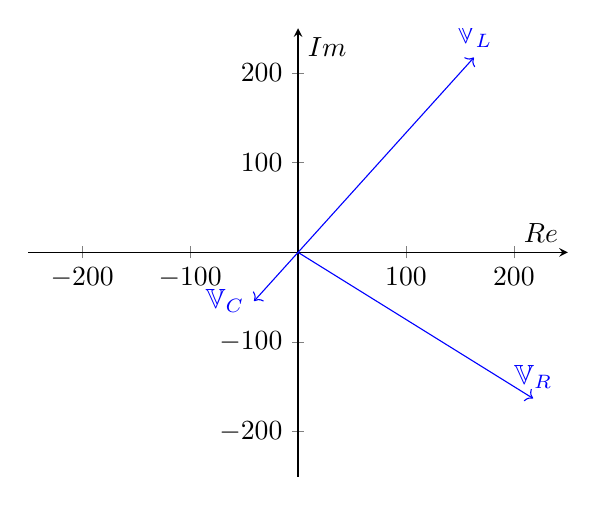
\begin{tikzpicture}
    		\begin{axis}[
    		xmin=-250,
    		xmax=250,
    		ymin=-250,
    		ymax=250,
    		axis lines = middle,
    		xlabel = $Re$,
    		ylabel = {$Im$}
    		]
    		
    		\addplot [blue, no markers, ->] coordinates {(0,0) (217.80,-162.92)} node[above,pos=1] {$\mathbb{V}_R$};
    		\addplot [blue, no markers, ->] coordinates {(0,0) (162.92,217.31)} node[above,pos=1] {$\mathbb{V}_L$};
    		\addplot [blue, no markers, ->] coordinates {(0,0) (-40.73,-54.32)} node[left,pos=1] {$\mathbb{V}_C$};
    		
    		\end{axis}
    		\end{tikzpicture}
    	\end{minipage}
    	\begin{minipage}{0.5\textwidth}
    		\begin{tikzpicture}
    		\begin{axis}[
    		xmin=-10,
    		xmax=10,
    		ymin=-10,
    		ymax=10,
    		axis lines = middle,
    		xlabel = $Re$,
    		ylabel = {$Im$}
    		]
    		
    		\addplot [red, no markers, ->] coordinates {(0,0) (5.43,-4.07)} node[above,pos=1] {$I$};
    		
    		\end{axis}
    		\end{tikzpicture}
    	\end{minipage}
    \end{figure}
    
	\newpage
	 
    \textbf{1.2.6}\\
    
    The analysis in this question allows for variable angular frequency, $\omega$. We first note that the impedance for $Z_1$ is given by:
    \begin{align*}
	    Z_1 = R
    \end{align*}
    
    The impedance for $Z_2$ is given by:
    \begin{align*}
	    Z_2 = j \omega L
    \end{align*}
    
    The impedance for $Z_3$ is given by:
    \begin{align*}
	    Z_3 = -j\frac{1}{\omega C}
    \end{align*}
    
    The equivalent impedance of the circuit is given by:
    \begin{align*}
	    Z_{eq} 	&= Z_1 + Z_2 + Z_3\\
			    &= R + j \omega L - j \frac{1}{\omega C}\\
			    &= R +j(\omega L - \frac{1}{\omega C})
    \end{align*}
    
    We can express the current using Ohm's law as follows:
    \begin{align*}
	    I 	&= \frac{V}{Z_{eq}}\\
		    &= \frac{V}{R + j(\omega L - \frac{1}{\omega C})}
    \end{align*}
    
    The magnitude of the current is given as:
    \begin{align*}
	    |I| = \frac{|V|}{\sqrt{(R)^2 + (\omega L - \frac{1}{\omega C})^2}}
    \end{align*}
    
    We note that both $V$ and $R$ are fixed and that the magnitude of the load current is only impacted by the change in the angular frequency. Hence, to maximise $I$, we want to find $\omega$ such that $(\omega L - \frac{1}{\omega C})^2$ is zero. Hence, the equation simplifies to:
    \begin{align*}
	    |I_{max}| 	&= \frac{|V|}{R}\\
				    &= \frac{339.41}{40}\\
				    &= 8.48\si{\ampere}
    \end{align*}
    
    
    Hence, we see that;
    \begin{center}
    	\fbox{$|I_{max}| = 8.48\si{\ampere}$}
    \end{center}
    \textbf{1.2.7}\\
    Building on the ideas presented in 1.2.6, we see that if we want the maximum current, then:
    \begin{align*}
    (\omega L - \frac{1}{\omega C})^2 	&= 0\\
    \omega L 							&= \frac{1}{\omega C}\\
    \omega^2							&= \frac{1}{LC}\\
    \omega								&= \frac{1}{\sqrt{LC}}
    \end{align*}
    
    Hence, we see that the angular frequency at which the load current is maximum is:
    \begin{center}
	    \fbox{$\omega = \frac{1}{127.324 \si{\milli\henry} \cdot 318.3 \si{\micro\farad}} = 24.67 \ \si{\kilo\radian\per\second} $}
	\end{center}
    
    \textbf{1.2.8}\\
    
    The frequency found in 1.2.7 is called the resonant frequency.\\
    
    \textbf{1.2.9}\\
    
    We know that the power factor is given by $\cos (\theta_{pf})$, and that $\theta_{pf} = \theta{v} - \theta_{i}$. Hence, we know that:
    \begin{align*}
	    \mathbb{I} = \frac{339.41 \angle 0 \si{\degree}}{40 + j \cdot (\omega L - \frac{1}{\omega C})}	    
    \end{align*}
    
    Hence, we can see that:
    \begin{align*}
	    \theta_{i} = - \arctan \bigg(\frac{1}{40} \cdot \bigg(\omega L - \frac{1}{\omega C}\bigg)\bigg)
    \end{align*}
    
    Therefore, the power factor is given by the following expression:
    \begin{align*}
	    \cos (\theta_{pf}) 	&= \cos \bigg( 0 - - \arctan \bigg(\frac{1}{40} \cdot \bigg(\omega L - \frac{1}{\omega C}\bigg)\bigg) \bigg)\\
						    &= \cos \bigg(\arctan \bigg(\frac{1}{40} \cdot \bigg(\omega L - \frac{1}{\omega C}\bigg)\bigg) \bigg)
    \end{align*}
    
    That is the power factor is:
    \begin{center}
    	\fbox{$\cos (\theta_{pf}) = \cos \bigg(\arctan \bigg(\frac{1}{40} \cdot \bigg(\omega L - \frac{1}{\omega C}\bigg)\bigg) \bigg)$}
    \end{center}
    
    \textbf{1.2.10}\\
    
    Geoffery. The source's name is Geoffery.\\
    
    Just kidding - I'm fairly certain that the only type of source that has a variable frequency is the function generators that we use in the laboratory.
\end{homeworkProblem}



%%%%%%%%%%%%%%%%%%%%%%%%%%%%%%%%%%%%%%%%%%%%%%%%%%%%%%%%%%%%%%%%%%%%%%%%%%%%%%%%%%%%%%%%%%%%%%%%%%%%%%%%%%%%%%%%%%%%%%
% Question 3
%%%%%%%%%%%%%%%%%%%%%%%%%%%%%%%%%%%%%%%%%%%%%%%%%%%%%%%%%%%%%%%%%%%%%%%%%%%%%%%%%%%%%%%%%%%%%%%%%%%%%%%%%%%%%%%%%%%%%%

\begin{homeworkProblem}
    
    A star-connected balanced three phase load is supplied from a balanced three phase source. Line voltage at the load is 415 $\si{\volt}$ and the line current is 20 $\si{\ampere}$ at a power factor of 0.8 lagging.\\
    
    \textbf{1.3.1}\\
    
    To determine the load impedance in each phase, we need to find the current in the phase and the voltage across the phase. If the line voltage $\mathbb{V}_{ab} = 415 \angle 0\si{\degree} \si{\volt}$, then the phase voltage is as follows:
    
    \begin{align*}
    \mathbb{V}_{AN} 	&= \frac{1}{\sqrt{3}} \cdot 415 \angle (0\si{\degree} - 30\si{\degree}) \si{\volt}\\
    &= 239.60 \angle -30 \si{\degree} \si{\volt}
    \end{align*}
    
    The power factor is 0.8 lagging, hence, the power factor angle $\theta_{pf}$, is given by:
    \begin{align*}
    \theta_{pf} = \cos^{-1}(0.8) = 36.86\si{\degree}
    \end{align*}
    
    The given that the current is lagging the voltage in the system, line current for the A phase is:
    \begin{align*}
    \mathbb{I}_{aA} = 20 \angle -36.86\si{\degree}
    \end{align*}
    
    Hence, we can find the load impedance as follows:
    \begin{align*}
    \mathbb{Z}_{A} = \frac{\mathbb{V}_{AN}}{\mathbb{I}_{aA}} = \frac{239.60 \angle -30 \si{\degree}}{20 \angle -36.86\si{\degree}} = 11.98 \angle 6.86 \si{\degree} \si{\ohm}
    \end{align*}
    
    Now, since the load is balanced, we know that:
    \begin{center}
    	\fbox{$\mathbb{Z}_A = \mathbb{Z}_B = \mathbb{Z}_C = 11.98 \angle 6.86 \si{\degree} \si{\ohm} = 11.98 + j1.43 \si{\ohm}$}
    \end{center}
    
    \textbf{1.3.2}\\
    
    If the load was in a $\Delta$-configuration, then we know that the line voltages are the same as the phase voltages and hence $\mathbb{V}_{ab} = \mathbb{V}_{AN} = 415 \angle 0 \si{\degree} \si{\volt}$. In the $\Delta$-configuration we know that the line currents and phase currents are different. Given our line current, $\mathbb{I}_{aA} = 20 \angle -36.86\si{\degree}$, which was derived above, we can find the phase current as follows:
    \begin{align*}
    \mathbb{I}_{AB} &= \frac{1}{\sqrt{3}} \cdot 20 \angle (-36.86 + 30)\si{\degree}\\
    &= 11.54 \angle -6.86\si{\degree}
    \end{align*}
    
    Hence, the impedance in the $\Delta$-configured load is:
    \begin{align*}
    \mathbb{Z}_{AB} = \frac{\mathbb{V}_{AB}}{\mathbb{I}_{AB}} = \frac{415 \angle 0 \si{\degree}}{11.54 \angle -6.86 \si{\degree}} = 35.96 \angle 6.86 \si{\degree} \si{\ohm}
    \end{align*}
    
    Since the load is balanced, we know that:
    \begin{center}
    	\fbox{$\mathbb{Z}_{AB} = \mathbb{Z}_{BC} = \mathbb{Z}_{CA} = 35.96 \angle 6.86 \si{\degree} \si{\ohm} = 35.70 + j4.30 \si{\ohm}$}
    \end{center}
	
\end{homeworkProblem}

%%%%%%%%%%%%%%%%%%%%%%%%%%%%%%%%%%%%%%%%%%%%%%%%%%%%%%%%%%%%%%%%%%%%%%%%%%%%%%%%%%%%%%%%%%%%%%%%%%%%%%%%%%%%%%%%%%%%%%
% Question 4
%%%%%%%%%%%%%%%%%%%%%%%%%%%%%%%%%%%%%%%%%%%%%%%%%%%%%%%%%%%%%%%%%%%%%%%%%%%%%%%%%%%%%%%%%%%%%%%%%%%%%%%%%%%%%%%%%%%%%%

\begin{homeworkProblem}
    Suppose that two watt meters were attached to the lines of a star, unbalance three phase load. Now watt meter 1 is measuring across the line A and the reference line, which is line B. The instantaneous power read from watt meter 1 is given by:
    \begin{align*}
	    W_1 = i_{aA} \cdot (V_{AN} - V_{BN})
    \end{align*} 
    
    Similarly, watt meter 2 is measuring the instantaneous power across line C, using line B as a reference:
    \begin{align*}
	    W_2 = i_{cC} \cdot (V_{CN} - V_{BN})
    \end{align*}
    
    Now, the total power is given by the following:
    \begin{align*}
	    P_{total} 	&= W_1 + W_2\\
				    &= i_{aA} \cdot (V_{AN} - V_{BN}) + i_{cC} \cdot (V_{CN} - V_{BN})\\
				    &= i_{aA} \cdot V_{AN} - i_{aA} \cdot V_{BN} + i_{cC} \cdot V_{CN} - i_{cC} \cdot V_{BN}\\
				    &= i_{aA} \cdot V_{AN} + i_{cC} \cdot V_{CN} - (i_{aA} + i_{cC}) \cdot V_{BN}\\
				    &= i_{aA} \cdot V_{AN} + i_{bB} \cdot V_{BN} + i_{cC} \cdot V_{CN}
    \end{align*}
  
	  Hence, the total instantaneous power absorbed by the three phase load can be measured by two watt meters, and the measurement is independent of whether the loads are balanced or unbalanced. 
\end{homeworkProblem}

%%%%%%%%%%%%%%%%%%%%%%%%%%%%%%%%%%%%%%%%%%%%%%%%%%%%%%%%%%%%%%%%%%%%%%%%%%%%%%%%%%%%%%%%%%%%%%%%%%%%%%%%%%%%%%%%%%%%%%
% Question 5
%%%%%%%%%%%%%%%%%%%%%%%%%%%%%%%%%%%%%%%%%%%%%%%%%%%%%%%%%%%%%%%%%%%%%%%%%%%%%%%%%%%%%%%%%%%%%%%%%%%%%%%%%%%%%%%%%%%%%%

\begin{homeworkProblem}
	A single phase 120 $\si{\volt}$, 60 \si{\hertz} supply is connected to a coil of 200 turns wound around a toroidal magnetic core with a mean length of 100$\si{\centi\meter}$, and a uniform cross section of 20 $\si{\centi\meter^2}$ and a relative permeability of 2500.\\
	
	\textbf{Part (a)}\\
	
	Assuming that we have received the voltage as an rms value, we first need to convert it:
	\begin{align*}
		V_m 	&= \sqrt{2} \cdot V_{rms}\\
				&= \sqrt{2} \cdot 120\\
				&= 169.71 \si{\volt}
	\end{align*}
	
	Further, we have to find the angular frequency:
	\begin{align*}
		\omega 	&= 2 \pi f\\
				&= 2 \pi \cdot 60\\
				& = 120 \pi
	\end{align*}
	
	Hence, the expression for the time varying voltage source is given by: $v(t) = 169.71 \cos(120 \pi t)$. To find the flux, $\phi$, we consider Faraday's law:
	\begin{align*}
		v(t) = N \cdot \frac{d \phi}{dt}\\
	\end{align*}
	
	Rearranging, we get:
	\begin{align}
		\frac{d \phi}{dt} = \frac{1}{N} \cdot 169.71 \cos(120 \pi t)
	\end{align}
	
	Given that $N = 200$, and taking the integral of both sides of (1):
	\begin{align*}
		\int \frac{d \phi}{dt} dt = \int_{0}^{t} \frac{1}{200} \cdot 169.71 \cos(120 \pi \tau) d\tau
	\end{align*}
	
	Simplifying, we get that:
	\begin{align*}
		\phi(t) 	&= \frac{169.71}{200} \cdot \bigg[\frac{1}{120 \pi} \cdot \sin (120 \pi t) \bigg]^{t}_{0}\\
					&= 2.25 \times 10^{-3} \cdot \sin (120 \pi t)
	\end{align*}
	
	Finally, we note that flux density, $B$, is simply flux divided by area:
	\begin{center}
		\fbox{$B = \frac{\phi (t)}{A} = 1.125 \sin(120 \pi t) \si{\tesla}$}
	\end{center}
	
	\textbf{Part (b)}\\
	
	To find the current, we note that: $B = \mu_0 \mu_r H$ and $F = Hl$. Now, magnetomotive force is given by $F = Ni$. Using the first formula, we note that:
	\begin{align*}
		H = \frac{B}{\mu_0 \mu_r}
	\end{align*}
	
	Then subbing this into the second equation, respectively:
	\begin{align*}
		F = \frac{Bl}{\mu_0 \mu_r}
	\end{align*}
	
	Rearranging the third equation and subbing in, we get that:
	\begin{align*}
		i 	&= \frac{Bl}{N \mu_0 \mu_r}\\
			&= \frac{1.125 \sin(120 \pi t) \cdot 1}{200 \cdot 4 \pi \times 10^{-7} \cdot 2500}\\
			&= 1.79 \sin(120 \pi t) \si{\ampere}
	\end{align*}
	
	Finally, the rms current is given by:
	\begin{center}
		\fbox{$i_{rms} = \frac{1.79}{\sqrt{2}} = 1.26\si{\ampere}$}
	\end{center}
\end{homeworkProblem}

%%%%%%%%%%%%%%%%%%%%%%%%%%%%%%%%%%%%%%%%%%%%%%%%%%%%%%%%%%%%%%%%%%%%%%%%%%%%%%%%%%%%%%%%%%%%%%%%%%%%%%%%%%%%%%%%%%%%%%
% Question 6
%%%%%%%%%%%%%%%%%%%%%%%%%%%%%%%%%%%%%%%%%%%%%%%%%%%%%%%%%%%%%%%%%%%%%%%%%%%%%%%%%%%%%%%%%%%%%%%%%%%%%%%%%%%%%%%%%%%%%%

\begin{homeworkProblem}
	For the series-parallel magnetic circuit made up of sheet steel, determine the current $I$ required to establish a flux of 0.2 $\si{\milli\weber}$ in the air gap. Given that $ab = bg = gh = ha = 0.2 \si{\meter}$, $bc = fg = 0.1 \si{\meter}$, $cd = ef = 0.099 \si{\meter}$, and the air gap is 0.002 $\si{\meter}$.\\
	
	\textbf{Part (a)}\\
	
	A simplified diagram of the magnetomotive force, $F$, which is driving the flux, $\Phi$, through the reluctances, $R$, can be seen below.
	
	\begin{figure}[h]
		\centering
		\ctikzset{bipoles/length=0.8cm}
		\begin{circuitikz}
			\draw
			(0,0) to [voltage source,l=$F$] (0,2)
			to [R,l=$R_{bahg}$, i_=$\Phi_1$] (2,2) 
			to [R, l=$R_{bg}$] (2,0) -- (0,0)
			(2,2) to [R,l=$R_{dcb}$,i_=$\Phi_2$] (4,2)
			to [R, l=$R_{gap}$] (4,0)
			to [R, l=$R_{efg}$] (2,0)
			;
		\end{circuitikz}
	\end{figure}
	
	Given that the constant of relative permeability is $\mu_r = 5570$, and that $\Phi_2 = 0.2 \times 10^{-3} \si{\weber}$, we can determine $F$ through linear circuit calculations. The first step is to calculate the reluctance values.
	
	\begin{align*}
		R_{gap} 	&= \frac{0.2}{4 \pi \times 10^{-7} \cdot 5 \times 10^{-4}} = 318.31 \times 10^4 \si{\ampere\per\weber}\\
		R_{bahg} 	&= 3 \cdot R_{ba} = \frac{3 \cdot 0.2}{5570 \cdot 4 \pi \times 10^{-7} \cdot 5 \times 10^{-4}} = 17.14 \times 10^4 \si{\ampere\per\weber}\\
		R_{bg} 		&= \frac{0.2}{5570 \cdot 4 \pi \times 10^{-7} \cdot 2 \times 10^{-4}} = 142.87 \times 10^4 \si{\ampere\per\weber}\\
		R_{dcb} 	&= R_{efg} = \frac{0.1 + 0.099}{5570 \cdot 4 \pi \times 10^{-7} \cdot 5 \times 10^{-4}} = 5.68 \times 10^4 \si{\ampere\per\weber}
	\end{align*}
	
	Now, taking a KVL around the right most loop above:
	\begin{align*}
		\Phi_2 \cdot (2 \cdot R_{dcb} + R_{gap} + R_{bg}) = \Phi_1 \cdot R_{bg}
	\end{align*}
	
	Rearranging, we get:
	\begin{align*}
		\Phi_1 	&= \frac{0.2 \times 10^{-3}}{142.87 \times 10^4} \cdot (2 \cdot 5.68 \times 10^4 + 318.31 \times 10^4 + 142.87 \times 10^4)\\
				&= 6.614 \times 10^{-4} \si{\weber}
	\end{align*}
	
	Now, taking a KVL around the leftmost loop gives the following equation:
	\begin{align*}
		-F + \Phi_1 \cdot R_{bahg} + (\Phi_1 - \Phi_2) \cdot R_{bg} = 0
	\end{align*}
	
	Rearranging, we can solve for $F$:
	\begin{align*}
		F 	&= \Phi_1 \cdot R_{bahg} + (\Phi_1 - \Phi_2) \cdot r_{bg}\\
			&= 6.614 \times 10^{-4} \cdot 17.14 \times 10^{4} + (6.614 \times 10^{-4} - 0.2 \times 10^{-3}) \cdot 142.87 \times 10^4\\
			&= 772.56 \si{\ampere t}
	\end{align*}
	
	Now, we know that $F = N \cdot i$, hence, rearranging to solve for $i$, given that $N = 200$ turns:
	\begin{center}
		\fbox{$i = \frac{F}{N} = \frac{772.56}{200} = 3.06 \si{\ampere}$}
	\end{center}
	
	
	\textbf{Part (b)}\\
	
	Consider the diagram below:
	
	\begin{figure}[h]
		\centering
		\ctikzset{bipoles/length=0.8cm}
		\begin{circuitikz}
			\draw
			(0,0) to [voltage source,l=$F$] (0,2)
			to [R,l=$F_{bahg}$, i_=$\Phi_T$] (2,2) 
			to [R, l=$F_{bg}$, i=$\Phi_2$] (2,0) -- (0,0)
			(2,2) to [R,l=$F_{dcb}$,i_=$\Phi_1$] (4,2)
			to [R, l=$F_{gap}$] (4,0)
			to [R, l=$F_{efg}$] (2,0)
			;
		\end{circuitikz}
	\end{figure}
	
	It is known that $\Phi_1 = 0.2 \times 10^{-3} \si{\weber}$. Hence, we find that:
	\begin{align*}
		B_{gap} = \frac{\Phi_1}{A} = \frac{0.2 \times 10^{-3}}{5 \times 10^{-4}} = 0.4 \si{\tesla}
	\end{align*}
	
	Therefore, it must be that:
	\begin{align*}
		H_{gap} = \frac{B_{gap}}{\mu_0} = \frac{0.4}{4 \pi \times 10^{-7}} = 318309.88 \si{\ampere t \per \meter}
	\end{align*}
	
	Finally, the \textit{mmf} can be found for the gap:
	\begin{align*}
		F_{gap} = H_{gap} \cdot l_{gap} = 318309.88 \times 0.002 = 636.61 \si{\ampere t}
	\end{align*}
	
	Similarly, we can find the \textit{mmf} for both $F_{bcd}$ and $F_{cfg}$. $B_{bcd} = 0.4 \si{\tesla}$, the same as the air gap, and using the $B-H$ curves, we find an $H_{bcd} = 70 \si{\ampere t \per \meter}$, approximately. Hence, we can find the \textit{mmf} as follows:
	\begin{align*}
		F_{bcd} = F_{efg} = H_{bcd} \cdot l_{bcd} = 70 \cdot (0.1 + 0.099) = 13.93 \si{\ampere t}
	\end{align*}
	
	Using a process similar to KVL, we find that:
	\begin{align*}
		F_{bg} = 2 \times 13.93 + 636.61 = 664.47 \si{\ampere t}
	\end{align*}
	
	Now, we can find what the field intensity is:
	\begin{align*}
		H_{bg} = \frac{F_{bg}}{l_{bg}} = \frac{664.47}{0.2} = 3322.35 \si{\ampere t \per \meter}
	\end{align*}
	
	Using the $B-H$ curves, we find that $B_{bg} = 1.56 \si{\tesla}$, approximately. From this we can find a value for $\Phi_2$:
	\begin{align*}
		\Phi_2 = B_{bg} \cdot A = 1.56 \cdot 2 \times 10^{-4} = 0.312 \si{\milli\weber}
	\end{align*}
	
	Using a process analogous to KCL, we can find a value for $\Phi_T$:
	\begin{align*}
		\Phi_T = \Phi_1 + \Phi_2 = 0.2 \times 10^{-3} + 0.312 \times 10^{-3} = 0.512 \si{\milli\weber}
	\end{align*}
	
	Hence, we can see that $B_{bahg}$:
	\begin{align*}
		B_{bahg} = \frac{0.512 \times 10^{-3}}{5 \times 10^{-4}} = 1.024 \si{\tesla}
	\end{align*}
	
	Using the $B-H$ sheets, we find that $H_{bahg} = 220 \si{\ampere t \per \meter}$. And the \textit{mmf} is given by:
	\begin{align*}
		F_{bahg} = 220 \cdot 3 \cdot 0.2 = 132 \si{\ampere t}
	\end{align*}
	
	Using a process analogous to KVL, we see that the total \textit{mmf} can be described as:
	\begin{align*}
		F = F_{bahg} + F_{bg} = 132 + 664.47 = 796.47 \si{\ampere t}
	\end{align*}
	
	Finally, we can find the current that is passing through the coil:
	\begin{center}
		\fbox{$i = \frac{F}{N} = \frac{796.47}{200} = 3.98 \si{\ampere}$}
	\end{center}
	
\end{homeworkProblem}

\end{document}
